\chapter{MSC: Diagramas de secuencia}
\label{ch:msc}

Según Bjorner~\cite{bjorner}, los diagramas de secuencia (a partir de
ahora MSCs), son una notación gráfica para describir intercambios de
mensajes entre entidades. Los MSCs fueron estandarizados por primera
vez por la \textit{CCITT} (conocida ahora como la \textit{ITU-T}) en
\textit{Recommendation Z.120} en 1992, donde se especificaron sus
componentes. Se realizaron revisiones en 1996, donde se especificó la
forma en que varios MSCs (llamados \textit{basic} MSC (BMSC) pueden
ser combinados para formar un documento MSC en cual la relación entre
dichos BMSCs se describe mediante un \textit{high-level} MSC (HMSC), y
en 1999 donde se ofrecen facilidades adicionales para la
especificación de los datos que se pasan dentro de los mensajes, y se
permiten expresiones en línea.

A continuación vamos a hacer un breve resumen sobre los BMSC, que son
los diagramas que vamos a usar en \textit{Progtalk}.

\section{Basic MSCs (BMSCs)}
Un \textit{basic} MSC (a partir de ahora BMSC), esta formado por un
conjunto de instancias. Una instancia es una entidad abstracta en la
cual suceden eventos. Una instancia se nota con un cuadrado vacío, el
cual tiene una linea recta que sale verticalmente y hacia abajo desde
su base. Esta recta representa una linea temporal donde los eventos
van ocurriendo por orden cronológico de arriba hacia abajo. Los
eventos que pueden suceder entre instancias son:

\subsection*{Acciones}
Son eventos locales a una instancia. Se representan por una caja en la
línea temporal con una etiqueta en su interior. Las acciones se usan
para especificar cambios en el estado interno de la instancia,
\subsection*{Mensajes salientes} 
Representan el envío de un mensaje desde una instancia origen a otra
instancia destino.
\subsection*{Mensajes entrantes}
Representan la recepción de un mensaje. Lógicamente a cada evento de
mensaje saliente le corresponde otro evento de mensaje entrante. A
esto se le conoce como \textit{intercambio de mensajes} y se representa con una
flecha que sale de la línea temporal de la instancia origen a la
línea temporal de la instancia destino. Todo intercambio de mensajes
debe de estar etiquetado con un identificador.
\subsection*{Condiciones}
Describen un estado el cual es común a un conjunto de instancias
dentro del MSC. Su fin es meramente informativo y se representan
mediante hexágonos los cuales se extienden a lo largo de las líneas de
tiempo de las instancias sobre las que la condición se aplica. El
texto de la condición debe ir en el interior del hexágono.
\subsection*{Temporizadores}
Estos eventos son locales a las instancias y como su propio nombre
indica sirven para controlar la ocurrencia temporal de los eventos. Se
nota con un reloj de arena.
\subsection*{Procesos de creación de instancias} 
Evento donde una instancia crea a otra nueva.
\subsection*{Procesos de terminación de instancias}
Evento donde una instancia se termina a si misma.
\subsection*{Corregiones} 
Son partes de la línea temporal de una instancia donde la premisa de
que los eventos ocurran de forma estrictamente temporal deja de ser
indispensable. Se notan con una línea discontinua.

En nuestro proyecto solo vamos a usar eventos de mensajes entrantes y
salientes. A continuación mostramos un ejemplo \ref{fig:fig1} de como
debería representarse gráficamente una comunicación.
\todo{AB:comprobar porque la fig1 no sale donde debiera.}

\begin{figure}
  \centering
  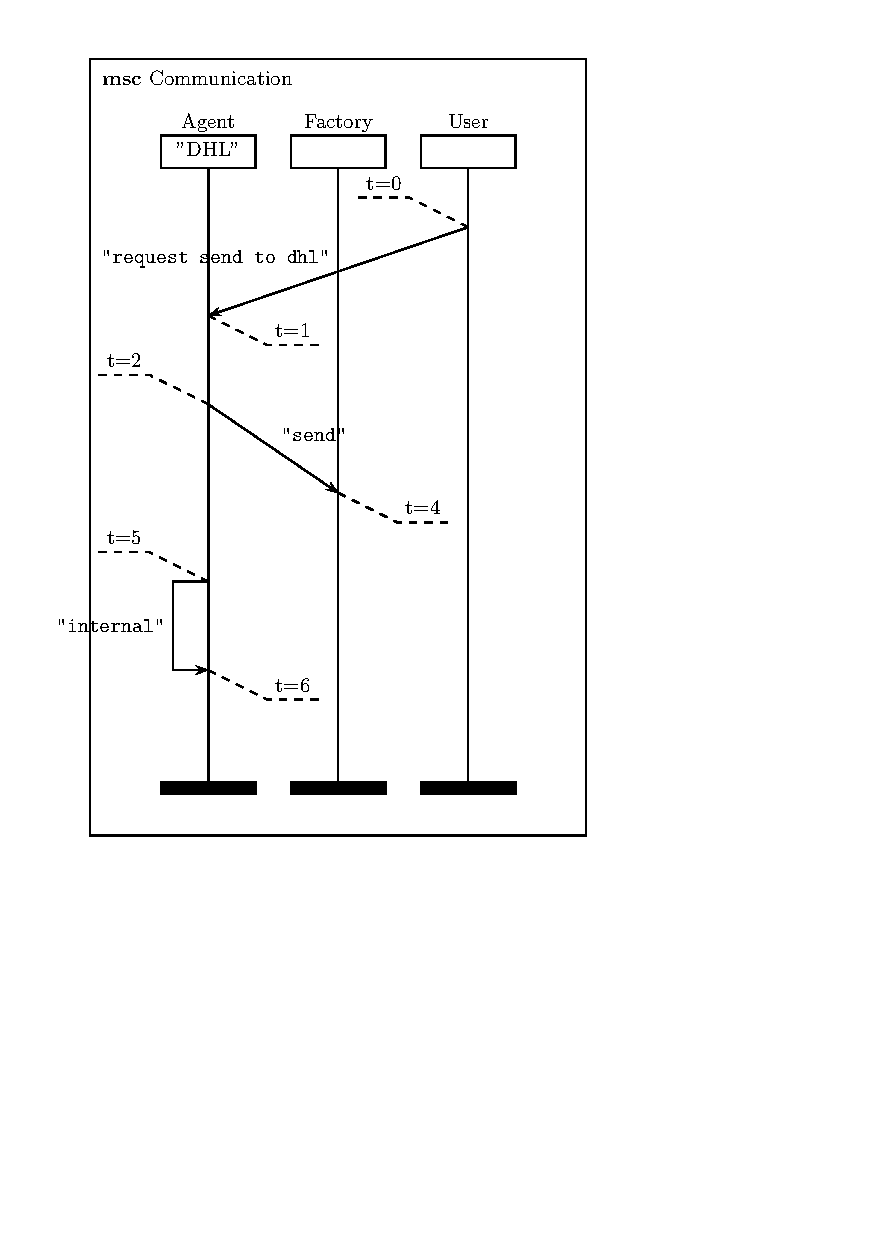
\includegraphics[scale=1]{./images/lars}
  \caption{Ejemplo de una comunicación generada con Progtalk}
  \label{fig:fig1}
\end{figure}

Para que nuestros BMSCs sean correctos deben cumplir una serie de requisitos:
\begin{itemize}
\item Los nombres de las instancias deben de ser únicos.
\item Todos los eventos de entrada y salida deben de estar
  relacionados con una instancia ya declarada en el momento del
  evento.
\item Los identificadores de los mensajes deben de ser únicos.
\item Un tiempo de envío no pueden ser nunca mayor que su
  correspondiente tiempo de recepción (ya que no podemos mandar un
  mensaje hacia atrás en el tiempo).
\end{itemize}


%%% Local Variables: 
%%% mode: latex
%%% TeX-master: "progtalk"
%%% TeX-PDF-mode: t
%%% ispell-local-dictionary: "castellano"
%%% End: 
